\documentclass[12pt]{article}
\usepackage[margin=1in]{geometry}
\usepackage{amsmath}
\usepackage{cancel}
\usepackage{tikz}
\usepackage{graphicx}
\setlength{\parskip}{0.3em}
\setlength{\parindent}{0pt}
% 使用系统字体,需要 XeLaTeX 或 LuaLaTeX 编译
\usepackage{fontspec}
\setmainfont{Times New Roman}
\usepackage{xcolor}
\usepackage{float}
\usepackage{caption}
\newcommand{\mdavg}[2]{\langle #1 \rangle\!\langle #2 \rangle}
\newcommand{\avg}[1]{\langle #1 \rangle}
\newcommand{\doubleavg}[2]{\left\langle #1 \right\rangle\!\left\langle #2 \right\rangle}
\newcommand{\inavg}[2]{\langle #1 \rangle\! [#2]}
\newcommand{\rinavg}[2]{[#1]\!\langle #2 \rangle}
\newcommand{\aket}[1]{|#1\rangle}
\newcommand{\asqu}[1]{{\langle#1\rangle}^2}
\newcommand{\sket}[1]{|#1]}
\newcommand{\cbrak}[2]{\avg{#1}\![#2]}
\newcommand{\acbrak}[2]{[#1]\!\avg{#2}}
\begin{document}

\title{Note for Scattering Amplitude Computation}
\author{Su Yingze}
\maketitle

\section{3-point building block}
We have known that the on-shell 3-point amplitudes can be completely determined by the little group scaling, according to the following formulas
\begin{align*}
    A_3^{h_1h_2h_3} &= c\avg{12}^{h_3-h_1-h_2}\avg{31}^{h_2-h_1-h_3}\avg{23}^{h_1-h_2-h_3}
    \quad & h_1+h_2+h_3 < 0 \\[0.5em]
    A_3^{h_1h_2h_3} &= c' [12]^{h_1+h_2-h_3}[23]^{h_2+h_3-h_1}[31]^{h_3+h_1-h_2}
    \quad & h_1+h_2+h_3 > 0
\end{align*}
Because of the specialty of this kind of 2 site gauge theory, there are no direct interaction between gauge boson and scalar, so there are only two kinds of 3-point amplitudes.
\begin{itemize}
    \item 2 scalar 1 gauge boson
    \begin{equation*}
        A[1,2,3^+]=\frac{[23][31]}{[12]},\qquad A[1,2,3^-]=\frac{\mdavg{23}{31}}{\avg{12}}
    \end{equation*}
    \item 3 gauge boson
    \begin{equation*}
        A[3^+,4^+,5^-]=\frac{[34]^3}{[45][53]},\qquad A[3^-,4^-,5^+]=\frac{\avg{34}^3}{\mdavg{45}{53}}
    \end{equation*}
\end{itemize}
If there are no exceptions, 1 and 2 always represent the antiscalar and scalar respectively, other number represent the gauge boson.  


\section{Gauge boson sector}
In this section, we will show how to build the gauge boson scattering. Because there's no direct interaction between gauge boson 1 and gauge boson 2, so we only need to compute one of them.
And although we have already known the formulas for MHV color-ordered amplitudes for gluon scattering -- Parke-Talyor Formula 
\begin{equation*}
    A[\cdots,i^-,\cdots,j^-,\cdots]=\frac{\avg{ij}^4}{\mdavg{12}{23}\cdots\mdavg{n-1,n}{n1}}
\end{equation*}
also for the anti-MHV amplitudes
\begin{equation*}
    A[\cdots,i^+,\cdots,j^+,\cdots]=\frac{[ij]^4}{[12][34]\cdots[n-1,n][n1]}
\end{equation*}
Here, we will give an concrete example to show how to use BCFW to compute the 4-point amplitudes $A[3^+,4^+,5^-,6^-]$

\begin{figure}[H]
    \centering
    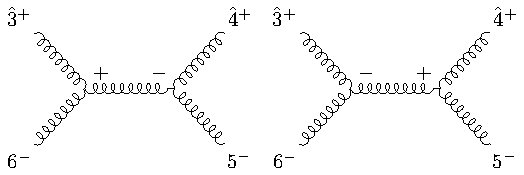
\includegraphics{4ptg.pdf}
    \caption*{4pt gluon}
\end{figure}
We choose the $[3,4\rangle$ shift, and it has been proved that $[+,+\rangle$ shift is valid
\begin{gather*}
    \sket{\hat{3}}=\sket{3}-z\sket{4},\qquad \qquad \aket{\hat{4}}=\aket{4}+z\aket{3}\\
    \aket{\hat{3}}=\aket{3}, \qquad \sket{\hat{4}}=\sket{4}.
\end{gather*}
The first diagram can be evaluated 
\begin{equation*}
    A_1=\frac{[\hat{3}\hat{I}]^3}{[\hat{I}6][6\hat{3}]}\times\frac{1}{s_{36}}\times\frac{\avg{5\hat{I}}^3}{\mdavg{\hat{I}\hat{4}}{\hat{4}5}}
\end{equation*}
The point here is that 
\begin{equation*}
    \text{Pole position}:\quad \hat{P}_{34}^2=0=\avg{36}[6\hat{3}]\quad \Rightarrow  \quad [6\hat{3}]=0,
\end{equation*}
for the similar reason, we can obtain $[\hat{I}6]=[6\hat{3}]=0$, so we conclude that the left part
\begin{equation*}
    \frac{[\hat{3}\hat{I}]^3}{[\hat{I}6][6\hat{3}]}=0
\end{equation*}
so the first channel is vanishing.

The second diagram can be similarly evaluated
\begin{align*}
    A_2&=\frac{\avg{\hat{I}6}^3}{\mdavg{6\hat{3}}{\hat{3}\hat{I}}}\times\frac{1}{s_{36}}\times\frac{[\hat{I}\hat{4}]^3}{[\hat{4}5][5\hat{I}]}\\
       &=\frac{[34]^3}{[34][45][56][61]}
\end{align*}
From this, we can conclude that the color-ordered amplitude equals to
\begin{equation*}
    A[3^+,4^+,5^-,6^-]=\frac{[34]^3}{[34][45][56][63]}.
\end{equation*}
and it can also be expressed by angle brackets interchangeably
\begin{equation*}
    A[3^+,4^+,5^-,6^-]=\frac{\avg{56}^3}{\mdavg{34}{45}\!\mdavg{56}{63}}
\end{equation*}
Then, 5-point , 6-point can be recursively computed by using BCFW recursion relation. 

\section{SQCD like sector}
\subsection{4-point case}
First we explain the color decomposition in this sector by 4 point amplitude $\Phi^\dagger V_1V_1\Phi$
    \begin{figure}[htbp]
        \centering
        \begin{minipage}[t]{0.32\textwidth}
            \centering
            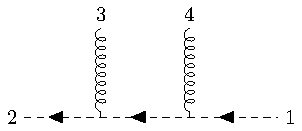
\includegraphics[width=\linewidth]{sch.pdf}
            \caption*{s channel}
        \end{minipage}
        \hfill
        \begin{minipage}[t]{0.32\textwidth}
            \centering
            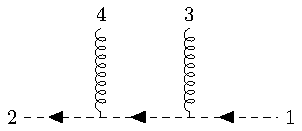
\includegraphics[width=\linewidth]{uch.pdf}
            \caption*{u channel}
        \end{minipage}
        \hfill
        \begin{minipage}[t]{0.32\textwidth}
            \centering
            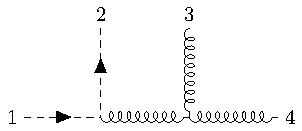
\includegraphics[width=\linewidth]{tch.pdf}
            \caption*{t channel}
        \end{minipage}
    \end{figure}

    The color factor can be written respectively as following
    \begin{equation*}
        r_s=\mathrm{Tr}[\Phi_2^\dagger T^{a_3}T^{a_4}\Phi_1],\,r_u=\mathrm{Tr}[\Phi_2^\dagger T^{a_4}T^{a_3}\Phi_1],\,
        r_t=\mathrm{Tr}[\Phi_2^\dagger [T^{a_3},T^{a_4}]\Phi_1]
    \end{equation*}
    We can easily obtain a similar Jacobbi relation
    \begin{equation*}
        r_t=r_s-r_u
    \end{equation*}
    Then we can accomplish the color decomposition and define the corressponding color-ordered amplitudes.

    For example, in the 4pt. case, the full amplitude can be decomposed to the following form
        \begin{align*}
            \mathcal{A}_4(\Phi^\dagger V_1V_1\Phi)&=A_s r_s+A_u r_u+A_t r_t\\
            &=A_s r_s+A_u r_u+A_t(r_s-r_u)\\
            &=(A_s+A_t)r_s+(A_u-A_t)r_u
        \end{align*}
        The two subamplitudes can be defined as color-ordered amplitude with order \textcolor{red}{[1,2,3,4]} and 
        \textcolor{red}{[1,2,4,3]} respectively.
        Of course, for the type $\Phi^\dagger(nV_1)\Phi$ and $\Phi (nV_2) \Phi^\dagger$, we can do the same thing to define the color-ordered amplitudes.

    We start from the 4-point color-ordered $A[1,2,3^+,4^-]$ again
    \begin{center}
    \begin{minipage}{0.45\textwidth}
        \begin{align*}
        A[1,2,3^+,4^-] &= \sum_{h}
        \end{align*}
        \end{minipage}
        \hspace{-3em}
        \begin{minipage}{0.45\textwidth}
        \raisebox{-1em}{\scalebox{0.8}{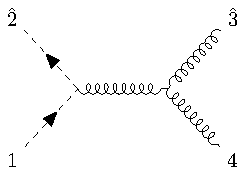
\includegraphics{4pt1.pdf}}}
        \end{minipage}
    \end{center}

    $\hspace{13.7em} =\raisebox{-2.5em}{\scalebox{0.7}{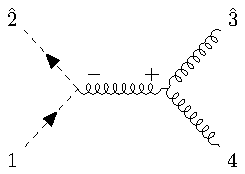
\includegraphics{4pt1.1.pdf}}}+\raisebox{-2.5em}{\scalebox{0.7}{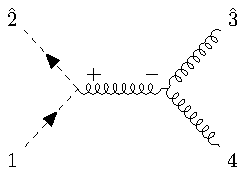
\includegraphics{4pt1.2.pdf}}}$

    For the same reason, the contribution from the second diagram is vanishing, so we only need to compute the firt one
    \begin{align*}
        A_1&=\frac{\avg{\hat{2}\hat{I}}\avg{\hat{I}1}}{\avg{1\hat{I}}}\times \frac{1}{s_{12}}\times \frac{[\hat{I}\hat{3}]^3}{[\hat{3}4][4\hat{I}]}\\
        &=(-1)\frac{\avg{14}^2\avg{24}^2}{\mdavg{12}{23}\!\mdavg{34}{41}}
    \end{align*}
    where we use the fact $\aket{\hat{2}}=\aket{2}$, $\sket{\hat{3}}=\sket{3}$, and the \textcolor{red}{Fierz Identity}
    \begin{equation*}
        [ij][kl]+[il][jk]+[ik][lj]=0
    \end{equation*}
    
    Here we can prove a nonus relation $\textcolor{red}{A[1,2,3^+,4^+]=0}$. Because of the vanishing of 3 gluon amplitude $A[+,+,+]$, so we only have one channel
    \begin{figure}[H]
        \centering
        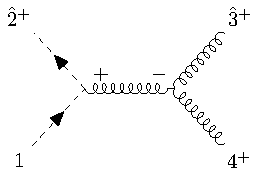
\includegraphics{4pt+.pdf}
        \caption*{all plus}
    \end{figure}

    Similarly, beacuse of the on-shell pole, we obtain
    \begin{equation*}
        [\hat{2}\hat{I}]=[\hat{I}1]=[1\hat{2}]=0,
    \end{equation*}
    so the contributaion from the left part
    \begin{equation*}
        \frac{[\hat{2}\hat{I}][\hat{I}1]}{[1\hat{2}]}=0,
    \end{equation*}
    then we can conclude that
    \begin{equation*}
        \textcolor{red}{A[1,2,3^+,4^+]=0}
    \end{equation*}
\subsection{5-point case}
Still, from the 4-point amplitude, we can first obtain 
\begin{equation*}
    \textcolor{red}{A[1,2,3^+,4^+,5^+]}.
\end{equation*}
For the 5-point MHV case, here we only consider the $(+,+,-)$ case. 
\begin{align*}
    A[1,2,3^+,4^+,5^+]&=\raisebox{-3em}{\scalebox{0.8}{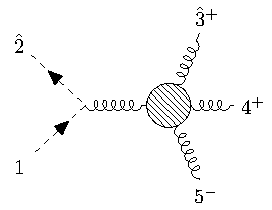
\includegraphics{5pt1.1.pdf}}}+\raisebox{-3em}{\scalebox{0.8}{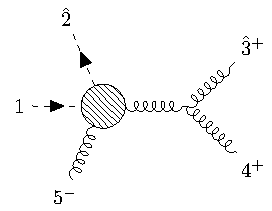
\includegraphics{5pt1.2.pdf}}}\\
    &=0+\frac{\avg{2\hat{5}}^2\avg{15}}{\avg{12}\!\mdavg{2\hat{I}}{\hat{I}5}}\times\frac{1}{s_{34}}\times\frac{[\hat{3}4]^3}{[4\hat{I}][\hat{I}3]}
\end{align*}
then we use
\begin{equation*}
    \cbrak{2\hat{I}}{\hat{I3}}=\cbrak{24}{43},\quad \acbrak{4\hat{I}}{\hat{I}5}=\acbrak{43}{\hat{3}5}
\end{equation*}
from the pole position
\begin{gather*}
    \hat{P}_{34}^2=0=\cbrak{\hat{3}4}{43}\quad \Rightarrow \quad \avg{\hat{3}4}=0\\
    \avg{34}+z\avg{24}=0\qquad\Rightarrow\quad z=-\frac{\avg{34}}{\avg{24}}
\end{gather*}
so
\begin{equation*}
    \avg{\hat{3}5}=\frac{\mdavg{32}{54}}{\avg{24}}
\end{equation*}
Then the color-ordered amplitude equals to 
\begin{equation*}
    A[1,2,3^+,4^+,5^+]=\frac{\avg{15}^2\avg{25}^2}{\mdavg{12}{23}\!\mdavg{34}{45}\!\avg{51}}
\end{equation*}
\subsection{n-point case}
It is not so hard to generallize these results to general case, here we only provide the compact formula, and the negligible sign are neglected
\begin{equation*}
    A[1,2,\cdots,n^-]=\frac{\avg{1,n}^2\avg{2,n}^2}{\mdavg{12}{23}\cdots\mdavg{n-1,1}{n,1}}
\end{equation*} 
\section{Pure 2-site sector}
\subsection{4-point case}
The color structure for this kind of amplitude has special form, like
\begin{equation*}
    (T_1^a)_{ij}(T_2^b)_{\bar{j}\bar{i}}
\end{equation*}
It is more straightforward to observe the color structure in terms of double line notation as follows 
\vspace{0.5em}

\tikzset{every picture/.style={line width=0.75pt}} %set default line width to 0.75pt        
\begin{center}
\begin{tikzpicture}[x=0.75pt,y=0.75pt,yscale=-1,xscale=1]
%uncomment if require: \path (0,300); %set diagram left start at 0, and has height of 300

%Straight Lines [id:da7604191870446242] 
\draw [color={rgb, 255:red, 255; green, 0; blue, 0 }  ,draw opacity=1 ]   (100,100) -- (150,100) ;
%Straight Lines [id:da7895005569652712] 
\draw [color={rgb, 255:red, 0; green, 110; blue, 237 }  ,draw opacity=1 ]   (100,110) -- (190,110) ;
%Straight Lines [id:da19217218880843812] 
\draw [color={rgb, 255:red, 255; green, 0; blue, 0 }  ,draw opacity=1 ]   (150,50) -- (150,100) ;
%Straight Lines [id:da7866299736623521] 
\draw [color={rgb, 255:red, 255; green, 0; blue, 0 }  ,draw opacity=1 ]   (160,50) -- (160,100) ;
%Straight Lines [id:da5667542352395977] 
\draw [color={rgb, 255:red, 0; green, 118; blue, 255 }  ,draw opacity=1 ]   (190,110) -- (190,160) ;
%Straight Lines [id:da33701635654582174] 
\draw [color={rgb, 255:red, 0; green, 118; blue, 255 }  ,draw opacity=1 ]   (200,110) -- (200,160) ;
%Straight Lines [id:da7076492571881566] 
\draw [color={rgb, 255:red, 255; green, 0; blue, 0 }  ,draw opacity=1 ]   (299,100) -- (389,100) ;
%Straight Lines [id:da3803886589182971] 
\draw [color={rgb, 255:red, 0; green, 113; blue, 255 }  ,draw opacity=1 ]   (200,110) -- (250,110) ;
\draw  [color={rgb, 255:red, 255; green, 4; blue, 37 }  ,draw opacity=1 ] (128,103.83) -- (120,100.45) -- (127.97,96.99) ;
\draw  [color={rgb, 255:red, 255; green, 4; blue, 37 }  ,draw opacity=1 ] (153.28,70.33) -- (150.12,78.42) -- (146.44,70.55) ;
\draw  [color={rgb, 255:red, 255; green, 4; blue, 37 }  ,draw opacity=1 ] (156.49,77.35) -- (160.07,69.44) -- (163.33,77.49) ;
\draw  [color={rgb, 255:red, 255; green, 4; blue, 37 }  ,draw opacity=1 ] (340,102.83) -- (332,99.45) -- (339.97,95.99) ;
\draw  [color={rgb, 255:red, 0; green, 119; blue, 255 }  ,draw opacity=1 ] (120.93,107.08) -- (128.98,110.35) -- (121.06,113.93) ;
\draw  [color={rgb, 255:red, 0; green, 119; blue, 255 }  ,draw opacity=1 ] (193.4,129.42) -- (190,137.42) -- (186.55,129.45) ;
\draw  [color={rgb, 255:red, 0; green, 119; blue, 255 }  ,draw opacity=1 ] (196.55,138.41) -- (200,130.44) -- (203.4,138.44) ;
\draw  [color={rgb, 255:red, 0; green, 119; blue, 255 }  ,draw opacity=1 ] (220.93,107.08) -- (228.98,110.35) -- (221.06,113.93) ;
%Straight Lines [id:da696489944746132] 
\draw [color={rgb, 255:red, 0; green, 113; blue, 255 }  ,draw opacity=1 ]   (300,110) -- (350,110) ;
\draw  [color={rgb, 255:red, 0; green, 119; blue, 255 }  ,draw opacity=1 ] (321,107) -- (329.05,110.27) -- (321.13,113.84) ;
%Straight Lines [id:da24340791537710427] 
\draw [color={rgb, 255:red, 0; green, 118; blue, 255 }  ,draw opacity=1 ]   (350,110) -- (350,160) ;
\draw  [color={rgb, 255:red, 0; green, 119; blue, 255 }  ,draw opacity=1 ] (353.4,129.42) -- (350,137.42) -- (346.55,129.45) ;
%Straight Lines [id:da7298898466192736] 
\draw [color={rgb, 255:red, 0; green, 118; blue, 255 }  ,draw opacity=1 ]   (360,110) -- (360,160) ;
\draw  [color={rgb, 255:red, 0; green, 119; blue, 255 }  ,draw opacity=1 ] (356.55,138.41) -- (360,130.44) -- (363.4,138.44) ;
%Straight Lines [id:da3460055698725] 
\draw [color={rgb, 255:red, 0; green, 110; blue, 237 }  ,draw opacity=1 ]   (360,110) -- (450,110) ;
\draw  [color={rgb, 255:red, 0; green, 119; blue, 255 }  ,draw opacity=1 ] (380.93,107.08) -- (388.98,110.35) -- (381.06,113.93) ;
%Straight Lines [id:da4507056480848969] 
\draw [color={rgb, 255:red, 255; green, 0; blue, 0 }  ,draw opacity=1 ]   (389,50) -- (389,100) ;
\draw  [color={rgb, 255:red, 255; green, 4; blue, 37 }  ,draw opacity=1 ] (393.28,70.33) -- (390.12,78.42) -- (386.44,70.55) ;
%Straight Lines [id:da6544383915955476] 
\draw [color={rgb, 255:red, 255; green, 0; blue, 0 }  ,draw opacity=1 ]   (399,50) -- (399,100) ;
\draw  [color={rgb, 255:red, 255; green, 4; blue, 37 }  ,draw opacity=1 ] (395.49,77.35) -- (399.07,69.44) -- (402.33,77.49) ;
%Straight Lines [id:da03624471669725382] 
\draw [color={rgb, 255:red, 255; green, 0; blue, 0 }  ,draw opacity=1 ]   (399,100) -- (449,100) ;
\draw  [color={rgb, 255:red, 255; green, 4; blue, 37 }  ,draw opacity=1 ] (427,103.83) -- (419,100.45) -- (426.97,96.99) ;
%Straight Lines [id:da34280653261510274] 
\draw [color={rgb, 255:red, 255; green, 0; blue, 0 }  ,draw opacity=1 ]   (160,100) -- (250,100) ;
\draw  [color={rgb, 255:red, 255; green, 4; blue, 37 }  ,draw opacity=1 ] (201,102.83) -- (193,99.45) -- (200.97,95.99) ;

% Text Node
\draw (255,97) node [anchor=north west][inner sep=0.75pt]   [align=left] {1};
% Text Node
\draw (81,97) node [anchor=north west][inner sep=0.75pt]   [align=left] {2};
% Text Node
\draw (165,46.4) node [anchor=north west][inner sep=0.75pt]    {$V_{1}$};
% Text Node
\draw (325,143.4) node [anchor=north west][inner sep=0.75pt]    {$V_{2}$};
% Text Node
\draw (407,47.4) node [anchor=north west][inner sep=0.75pt]    {$V_{1}$};
% Text Node
\draw (285,97) node [anchor=north west][inner sep=0.75pt]   [align=left] {2};
% Text Node
\draw (454,95) node [anchor=north west][inner sep=0.75pt]   [align=left] {1};
% Text Node
\draw (166,142.4) node [anchor=north west][inner sep=0.75pt]    {$V_{2}$};


\end{tikzpicture}
\end{center}
For the four point case $\mathcal{A}(V_2\Phi^\dagger V_1 \Phi )$, we can construct the color-ordered amplitude from the residue. First, we consider the $(+,-)$ helicity
configuration. There are two feynman diagrams contributing to the color-ordered amplitude.\\
\begin{figure}[htbp]
    \centering
    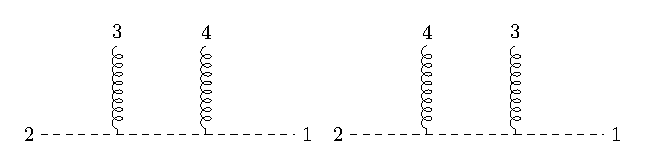
\includegraphics{4pt.eps}
    \caption{4pt.}
    \label{1}
\end{figure}

For the first diagram, the residue equals to
\begin{equation*}
    \mathcal{R}es|_{s_{12}=0}=\frac{[3 I ] [23]}{[I2]}\times \frac{\avg{I4}\avg{41}}{\avg{1I}}=\frac{\avg{24}[31]\avg{41}[23]}{[42]\avg{24}}
\end{equation*}
Similarly, the second one is
\begin{equation*}
    \mathcal{R}es|_{s_{13}=0}=\frac{\avg{4I}\avg{24}}{\avg{I2}}\times \frac{[31] [I3]}{[1I]}=\frac{\avg{24}[31]\avg{41}[23]}{\avg{32}[23]}
\end{equation*}

Then we can conclude that the four-point color-ordered amplitude $A[1,2,3^+,4^-]$ equals to
\begin{equation*}
    A[1,2,3^+,4^-]=\frac{\avg{24}[31]\avg{41}[23]}{\avg{32}[23][42]\avg{24}}=\frac{\avg{24}\avg{14}}{\avg{13}\avg{23}}
\end{equation*}

\textcolor{red}{$\star Bonus$}

It is still necessary to prove the color-ordered amplitude $A[1,2,3^+,4^+]$ equals to 0. Here we can use the color ordered Feynman rules to show the result.
\begin{equation*}
    A[1,2,3^+,4^+]\propto \frac{\left(\epsilon_3\cdot p_2\right)\left(\epsilon_4\cdot p_1\right)}{s_{23}}+\frac{\left(\epsilon_4\cdot p_2\right)\left(\epsilon_3\cdot p_1\right)}{s_{24}} 
\end{equation*}
Here we can utilize the spinor-helicity variable to express polarization vector
\begin{equation*}
    \epsilon_2^{+\mu}=\frac{\langle r_1 | \gamma^\mu | 3 ]}{\sqrt{2}\avg{r_13}},\qquad \epsilon_4^{+\mu}=\frac{\left <r_2|\gamma^\mu|4\right ]}{\sqrt{2}\avg{r_24}}
\end{equation*}
here $r_1$ and $r_2$ represent the reference spinor.

We can freely choose $r_1=r_2=1$ or 2, then $\avg{r_1 2}$,$\avg{r_2 1}$,$\avg{r_1 1}$,$\avg{r_2 2}$, two of them equal to 0, so we can conclude that
\begin{equation*}
    A[1,2,3^+,4^+]=0
\end{equation*}
\subsection{5-point case}
For the 5-point case, we can utilize the BCFW recursion relation which can help us generate higher point amplitude from lower point on-shell subamplitudes. Here, 
we always consider the MHV (Maximal helicity violation) amplitude. 
\par
If there is no special case, we always choose the following BCFW shift
\begin{gather*}
    \sket{\hat{2}}=\sket{2}-z\sket{3},\qquad \qquad \aket{\hat{3}}=\aket{3}+z\aket{3}\\
    \aket{\hat{2}}=\aket{2}, \qquad \sket{\hat{3}}=\sket{3}
\end{gather*}
where 2 always refers to antiscalar and 3 refers to gauge boson with + helicity.
\par
Let us begin with the simplest case $A[1,2,3_1^+,4_1^+,5_2^-]$, where the subscript represent which gauge group the particle belongs to. Because of the property 
of this kind of gauge theory, the color structure is invariant under the OPP (Order Preserving Permutation), in this case, for example,
\begin{equation*}
    (3_1^+,4_1^+,5_2^-)\qquad (3_1^+,5_2^-,4_1^+)\qquad(5_2^-,3_1^+,4_1^+)
\end{equation*}
give us the same color factor. So in the process of BCFW recursion, these three order offer the same amplitude. We can draw all diagrams contributing to the BCFW process, the first two are following
\par
\begin{figure}[H]
    \centering
    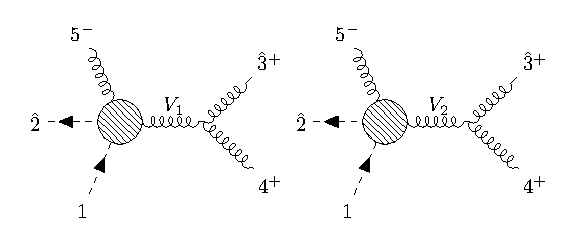
\includegraphics{5pt1.eps}
    \caption{5pt. 1}
    \label{2}
\end{figure}
It is obvious that the second diagram in Figure 2 equals to 0, because there are no interaction between the two gauge bosons.
\par
Similarly, another two diagrams equal to 0 for the same reason
\begin{figure}
    \centering
    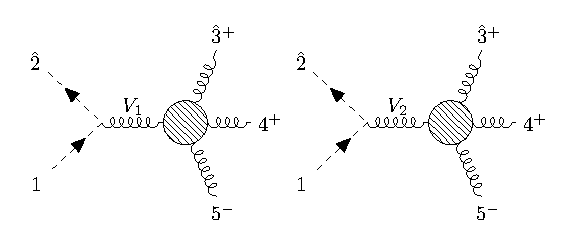
\includegraphics{5pt2.eps}
    \caption{5pt. 2}
    \label{3}
\end{figure}
\par
The last diagram still gives 0 contribution because it includes a subamplitude $A[1,\hat{I},\hat{3}^+,4^+]=0$.
\par
\begin{figure}[H]
    \centering
    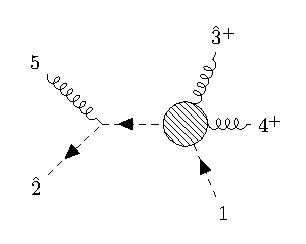
\includegraphics{5pt3.eps}
    \caption{5pt. 3}
    \label{4}
\end{figure}
Above all. only the first diagram in Figure 1 has non-vanishing contributions, so the full color ordered amplitude equals to
\begin{align*}
    A[1,2,3_1^+,4_1^+,5_2^-]&=A[1,2,\hat{I}^+,5^-]\times\frac{1}{s_{34}}\times A[\hat{3}^+,4^+,\hat{I}^-]\\
    &=\frac{\doubleavg{15}{25}}{\mdavg{1\hat{I}}{2\hat{I}}}\times\frac{1}{s_{34}}\times\frac{[\hat{3}4]^3}{[4\hat{I}][\hat{I}\hat{3}]}\\
    &=\frac{\mdavg{15}{25}\bcancel{[34]^3}}{\mdavg{14}{23}\avg{43}\bcancel{[43][43][34]}}\\
    &=\frac{\mdavg{15}{25}}{\mdavg{23}{34}\avg{41}}\\
    &=\frac{(-1)\avg{2\textcolor{green}{5}}^2\!\avg{1\textcolor{green}{5}}^2}{\textcolor{blue}{\mdavg{23}{34}\!\avg{41}}\textcolor{red}{\mdavg{25}{51}}}
\end{align*}
where we use the fact $|\hat{3}\rangle=|\hat{3}\rangle$ and following identities
\begin{equation*}
    \inavg{1\hat{I}}{\hat{I}3}=\inavg{14}{43},\quad \inavg{2\hat{I}}{\hat{I}3}=\inavg{24}{43}
\end{equation*}
and also
\begin{align*}
    \frac{[\hat{I}3]}{[4\hat{I}]}&=-\frac{\rinavg{3\hat{I}}{\hat{I}2}}{\rinavg{4\hat{I}}{\hat{I}2}}=-\frac{\rinavg{34}{42}}{\rinavg{43}{\hat{3}2}},\quad(\avg{\hat{3}2}=\avg{32}+z\avg{22}=\avg{32})\\
    &=\frac{\avg{42}}{\avg{32}}
\end{align*}
here green refers to the particle with (-) helicity, red refers to particles belong to gauge group 1, red refers to particles belong to gauge group 2.
\par
Similarly, it is very easy to obtain another color-ordered amplitude $A[1,2,3_1^+,4_1^-,5_2^+]$
\begin{align*}
    A[1,2,3_1^+,4_1^-,5_2^+]=
    \frac{(-1)\avg{2\textcolor{green}{4}}^2\!\avg{1\textcolor{green}{4}}^2}{\textcolor{blue}{\mdavg{23}{34}\!\avg{41}}\textcolor{red}{\mdavg{25}{51}}}
\end{align*}
and also $A[1,2,3_1^-,4_1^+,5_2^+]$ equals to
\begin{equation*}
    A[1,2,3_1^-,4_1^+,5_2^+]=
    \frac{(-1)\avg{2\textcolor{green}{3}}^2\!\avg{1\textcolor{green}{3}}^2}{\textcolor{blue}{\mdavg{23}{34}\!\avg{41}}\textcolor{red}{\mdavg{25}{51}}}
\end{equation*}
But here we need to emphasize that it is necessary to choose another BCFW shift, like $[1,5^+ \rangle$, as $[2,3^- \rangle$ is not a valid shift. 
\subsection{6-point case}
Here we consider $(V_2V_2\Phi^\dagger V_1V_1 \Phi)$ case, the corresponding color-ordered amplitude is $A[1,2,3_1^+,4_1^+,5_2^+,6_2^-]$.
Similarly, the fowwling orders all give us the same color factor
\begin{gather*}
    (3_1^+,4_1^+,5_2^+,6_2^-)\qquad(3_1^+,5_2^+,4_1^+,6_2^-)\qquad (3_1^+,5_2^+,6_2^-,4_1^+)\\
    (5_2^+,3_1^+,4_1^+,6_2^-)\qquad(5_2^+,3_1^+,6_2^-,4_1^+)\qquad (5_2^+,6_2^-,3_1^+,4_1^+)
\end{gather*}
Only two diagrams have semmingly non-zero contributaion,
\par
\begin{figure}[H]
    \centering
    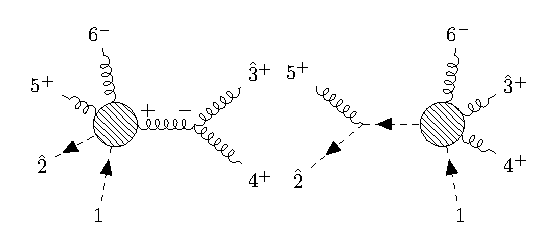
\includegraphics{6pt.eps}
    \caption{6pt.}
    \label{5}
\end{figure}
so the full color ordered amplitude equals to
\begin{align*}
    A_1&=\frac{(-1)\asqu{\hat{2}6}\asqu{16}}{\mdavg{25}{56}\!\avg{61}\!\mdavg{\hat{2}\hat{I}}{\hat{I}1}}\times\frac{1}{s_{34}}\times\frac{[\hat{3}4]^3}{[4\hat{I}][\hat{I}\hat{3}]}\\
    &=\frac{\asqu{26}\avg{16}}{\mdavg{25}{56}\!\mdavg{\hat{2}\hat{I}}{\hat{I}1}}\times\frac{1}{s_{34}}\times\frac{[34]^3}{[4\hat{I}][\hat{I}3]}\\
    &=\frac{\asqu{26}\avg{16}\bcancel{[34]^3}\bcancel{\avg{42}}}{\mdavg{25}{56}\!\mdavg{41}{32}\!\avg{43}\bcancel{[43][43][34]}\bcancel{\avg{24}}}\\
    &=\frac{\asqu{26}\!\asqu{16}}{\textcolor{blue}{\mdavg{23}{34}\!\avg{41}}\!\textcolor{red}{\mdavg{25}{56}\!\avg{51}}}
\end{align*}
where we have used the fact $\aket{\hat{2}}=\aket{2}$, $\sket{\hat{3}}=\sket{3}$, and the following identities
\begin{equation*}
    \inavg{2\hat{I}}{\hat{I}3}=\inavg{24}{43}, \qquad \rinavg{4\hat{I}}{\hat{I}1}=\rinavg{43}{\hat{3}1}
\end{equation*}
The point here is that we first $\avg{\hat{3}1}$ which does not appear in 5-point case, so we nned to compute it carefully
\begin{gather*}
    \text{pole position}: \quad \hat{P_{34}}^2=0=2P_3\cdot P_4=\inavg{4\hat{3}}{34}\qquad\Rightarrow \qquad \avg{4\hat{3}}=0\\
    \avg{43}+z\avg{42}=0\qquad \Rightarrow \qquad z=-\frac{43}{42}
\end{gather*}
then
\begin{align*}
    \avg{\hat{3}1}=\avg{31}+z\avg{21}&=\avg{31}-\frac{\avg{43}}{\avg{42}}\avg{21}\\
    &=\frac{\mdavg{42}{31}-\mdavg{43}{21}}{42}\\
    &=\frac{\mdavg{41}{32}}{\avg{42}}
\end{align*}
where we have used the Fierz identity
\begin{equation*}
    \mdavg{42}{31}+\mdavg{41}{23}+\mdavg{43}{12}=0.
\end{equation*}
Simiraly, we can compute the second diagram
\begin{equation*}
    A_2=\frac{[\hat{2}5][5\hat{I}]}{[\hat{I}\hat{2}]}\times\frac{1}{s_{25}}\times \frac{(-1)\asqu{16}\asqu{\hat{I}6}}{\mdavg{\hat{I}\hat{3}}{\hat{3}4}
    \!\mdavg{41}{\hat{I}6}\!\avg{61}}
\end{equation*}
but from the pole position
\begin{equation*}
    \hat{P_{25}}^2=0=2P_2\cdot P_5=\inavg{52}{\hat{2}5}\qquad\Rightarrow \qquad [\hat{2}5]=0,
\end{equation*}
and simiraly
\begin{equation*}
    [\hat{2}\hat{I}]=[5\hat{I}]=0.
\end{equation*}
Then we can conclude that the left part of the amplitude equals to 0 so $A_2=0$. Finally, we obtain the color-ordered amplitude 
\begin{equation*}
    A[1,2,3_1^+,4_1^+,5_2^+,6_2^-]=A_1+A_2=\frac{\asqu{26}\!\asqu{16}}{\textcolor{blue}{\mdavg{23}{34}\!\avg{41}}\!\textcolor{red}{\mdavg{25}{56}\!\avg{51}}}.
\end{equation*}
\subsection{n-point case}
Here, we first propose a compact formula for the color-ordered amplitude
\begin{equation*}
    A=\frac{\asqu{2a}\!\asqu{1a}}{\underbrace{\avg{2\star}\cdots \avg{\star 1}}_{SU(N_1)}\underbrace{\avg{2\ast }\cdots \avg{\ast 1}}_{SU(N_2)}}
\end{equation*}
where a refer to the particle with - helicity, whichever gauge group it belongs to. And, `$\star$' refers to the ordering for the first gauge group, `$\ast$'
refers to the ordering for the second gauge group. We suppose there are $n_1$ gauge boson 1, $n_2$ gauge boson 2, so the n-point means that $n=n_1+n_2+2$.
\par
The usual way to prove this kind of compact formula is deduction. First we suppose that all of the amplitudes with external point lower than n satisfy the compact formula.
And although there are $\frac{(n_1+n_2)!}{n_1!n_2!}$ OPP, we just need to consider some of them. 
\end{document}